\begin{figure}[H]
\begin{subfigure}{.6\textwidth}
\centering
\begin{class}{ActiveShop(id: \integer)}
\\
\begin{state}
self, vmId, message: \integer
\\transferableOperation: nil | talk
\end{state} 
\\
\begin{init}
\\self = id
\\transferableOperation = talk
\end{init} 
\\
\begin{op}{switch\_\_\_\_\ then\ IdleShop}
x!: nil | talk
\ST
x! = transferableOperation
\\transferableOperation' = nil
\end{op}
\\
\begin{op}{talk}
\Delta (vmId, message)
\\y?, z?: \integer
\ST
y? = message'
\\z? = vmId'
\end{op}
\end{class}
  \caption{ActiveShop OZ class}
\end{subfigure}%
\begin{subfigure}{.4\textwidth}
  \centering
\fbox{  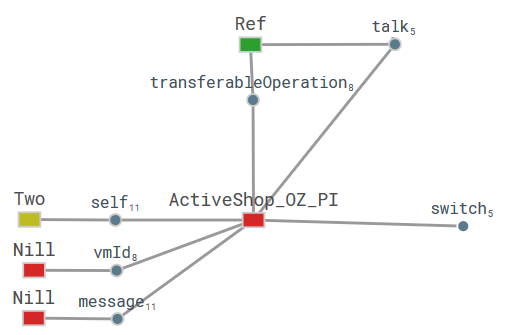
\includegraphics[width=.91\linewidth]{./images/transformational_semantics_of_oz/activeShop_OZ.png}}
  \caption{stargazer visualization}
\end{subfigure}
\caption{transforming ActiveShop into \picalc{} process ActiveShop\_OZ}
\label{tra_activeShop_OZ}
\end{figure}

\lstinputlisting[backgroundcolor=\color{white},caption={ ActiveShop OZ class as a process in ABC code.},captionpos=b, label={tra_activeShop_OZ_listing}]{listings/activeShop_OZ.abc}